
\begin{tcbdoublebox}[title={1. Eager Beaver and Eager Beaver}]
\mdseries Giả sử với trường hợp cả hai nhân vật Romeo và Juliet đều là Eager Beaver. Theo định nghĩa, Eager Beaver là một người được thúc đẩy bởi cảm xúc của chính mình và bởi tình yêu của đối phương dành cho anh ấy/cô ấy. Nói cách khác, tình yêu của Romeo dành cho Juliet càng tăng khi Juliet cành yêu anh ta và chính anh ta cũng phải yêu Juliet. Đối với Juliet thì cũng tương tự vậy. Ở đây ta xét đến hai ví dụ IVP ODEs Sys:\\
\bfseries Ví dụ 1: \\
\textcolor{blue}{$$\left\{\begin{matrix}
\dot{R} =  2R +3J \\ 
\dot{J} =  4R+2J\\ 
R(0)= -3, J(0)=-2
\end{matrix}\right.$$}\\
\mdseries Ma trận $\color{blue}A=\begin{pmatrix}
2 & 3\\ 
4 & 2
\end{pmatrix}$ có hai trị riêng là 
$\color{blue}\lambda_{1}=2+2\sqrt{3};\ \lambda_{2}=2-2\sqrt{3}$
, lần lượt tương ứng với các vecto riêng:
$\color{blue}v_{1} = (\sqrt{3}; 2)^{T};\ v_{2}=(\sqrt{3}; -2)^{T}$\\Áp dụng công thức bài tập 1, nghiệm của hệ phương trình là:
$$R(t)=-\frac{{\mathrm{e}}^{2\,t\,\left(\sqrt{3}+1\right)}\,\left(\sqrt{3}+3\right)}{2}-\frac{\sqrt{3}\,{\mathrm{e}}^{-2\,t\,\left(\sqrt{3}-1\right)}\,\left(\sqrt{3}-1\right)}{2} $$
$$J(t)={\mathrm{e}}^{-2\,t\,\left(\sqrt{3}-1\right)}\,\left(\sqrt{3}-1\right)-\frac{\sqrt{3}\,{\mathrm{e}}^{2\,t\,\left(\sqrt{3}+1\right)}\,\left(\sqrt{3}+3\right)}{3}$$
\\
\bfseries Ví dụ 2: \\
$$\color{blue}\left\{\begin{matrix}
\dot{R} =  3R + 2J \\ 
\dot{J} =  1R + 2J\\
R(0)= 3, J(0)=-2
\end{matrix}\right.$$
\mdseries Ma trận $\color{blue}A=\begin{pmatrix}
3 & 2\\ 
1 & 2
\end{pmatrix}$ có hai trị riêng lần lượt là $\color{blue}\lambda_{1}=4;\ \lambda_{2}=1$
, lần lượt tương ứng với các vecto riêng:
$\color{blue}v_{1} = (2;\ 1)^{T};\ v_{2}=(-1;\ 1)^{T}$
\\
Áp dụng công thức bài tập 1, nghiệm của hệ phương trình là:
$$R(t)=\frac{2\,{\mathrm{e}}^{4\,t}}{3}+\frac{7\,{\mathrm{e}}^t}{3} $$
$$J(t)=\frac{{\mathrm{e}}^{4\,t}}{3}-\frac{7\,{\mathrm{e}}^t}{3}$$

\textbf{Nhận xét: } Như đã nói, vì cả hai đều là Eager Beaver, nên tình cảm của cả hai sẽ phụ thuộc vào chính họ và đối phương. Thế nên trong \textbf{Ví dụ 1} khi mà thời điểm ban đầu cả hai đều ghét nhau thì theo thời gian tình cảm của họ sẽ ngày càng giảm đi, còn trong \textbf{Ví dụ 2} ban đầu dù có một bên ghét thế nhưng các chỉ số a,b,c,d sẽ kéo tình cảm này lên dương vào một thời điểm nào đó và khi thời gian đủ lớn, tình cảm cả hai cũng ngày càng tăng lên. 

Hai cặp \textbf{đồ thị plot và phase portrait} dưới đây sẽ mô tả cho điều này!
\end{tcbdoublebox}
\pagebreak
\begin{figure}[!htbp]
    \centering
    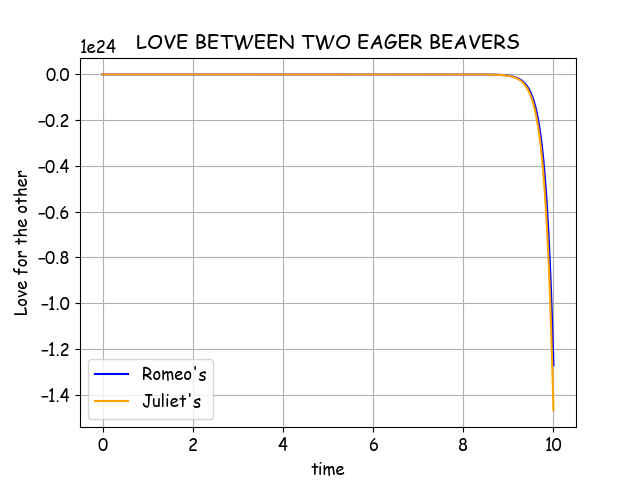
\includegraphics[width=100mm]{image/bt2/plot1.1.png}
    \caption{VD1.1 - The plot of the love between two eager beavers }
\end{figure}
\begin{figure}[!htbp]
    \centering
    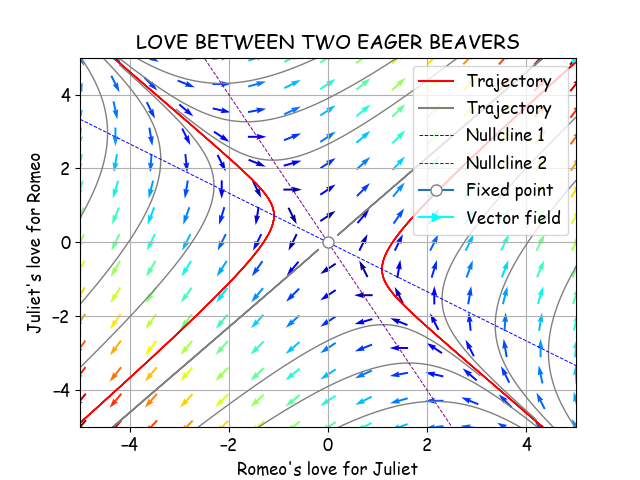
\includegraphics[width=100mm]{image/bt2/pp1.1.png}
    \caption{VD1.1 - The phase portrait of the love between two eager beavers}
\end{figure}

\textbf{Dạng Phase portrait: } Saddle
\pagebreak
\begin{figure}[!htbp]
    \centering
    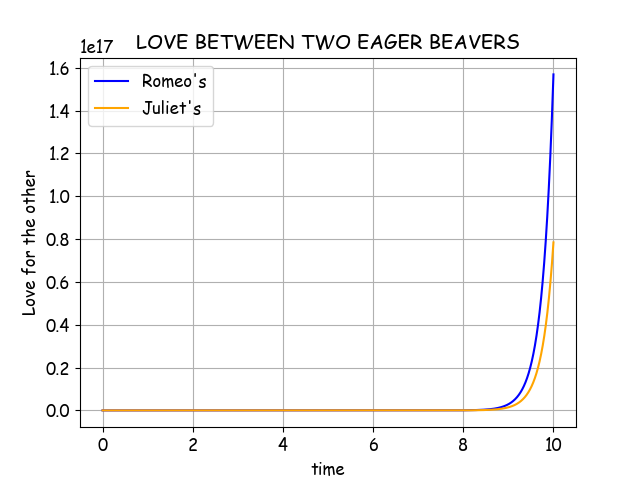
\includegraphics[width=100mm]{image/bt2/plot1.2.png}
    \caption{VD1.2 - The plot of the love between two eager beavers}
\end{figure}
\begin{figure}[!htbp]
    \centering
    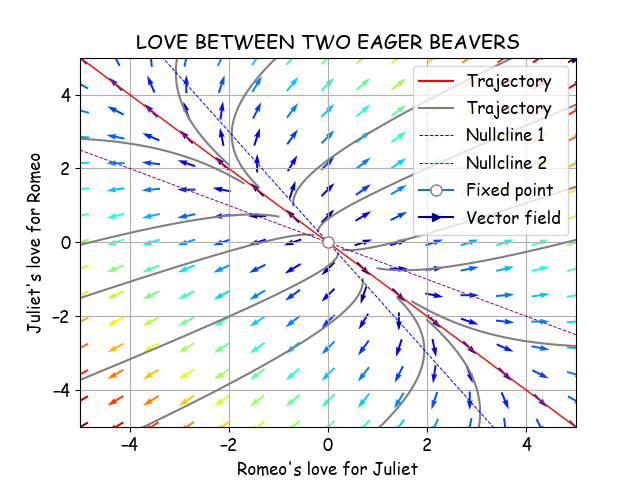
\includegraphics[width=100mm]{image/bt2/pp1.2.png}
    \caption{VD1.2 - The phase portrait of the love between two eager beavers}
\end{figure}

\textbf{Dạng Phase portrait: } Nodal Source
\pagebreak

%%%%%%%%%%%%%%%%%%2222222222%%%%%%%%%%%%%%%%%%%%%%%%
%%%%%%%%%%%%%%%%%%%%%%%%%%%%%%%%%%%%%%%%%%%%%%%%%%%%%
\begin{tcbdoublebox}[title={2. Narcissistic Nerd and Narcissistic Nerd}]
\mdseries .\\
\bfseries Ví dụ 1: \\
\textcolor{blue}{$$\left\{\begin{matrix}
\dot{R} =  2R -3J \\ 
\dot{J} =  -4R+3J\\ 
R(0)= 3, J(0)=-2
\end{matrix}\right.$$}\\
\mdseries Ma trận $\color{blue}A=\begin{pmatrix}
2 & -3\\ 
-4 & 3
\end{pmatrix}$ có hai trị riêng là 
$\color{blue}\lambda_{1}=-1;\ \lambda_{2}=6$
, lần lượt tương ứng với các vecto riêng:
$\color{blue}v_{1} = (1;\ 1)^{T};\ v_{2}=(-3;\ 4)^{T}$\\Áp dụng công thức bài tập 1, nghiệm của hệ phương trình là:
$$R(t)=\frac{6\,{\mathrm{e}}^{-t}}{7}+\frac{15\,{\mathrm{e}}^{6\,t}}{7} $$
$$J(t)=\frac{6\,{\mathrm{e}}^{-t}}{7}-\frac{20\,{\mathrm{e}}^{6\,t}}{7}$$
\\
\bfseries Ví dụ 2:\\
\textcolor{blue}{$$\left\{\begin{matrix}
\dot{R} =  4R + -4J \\ 
\dot{J} =  -4R + 4J\\ 
R(0)= \frac{5}{2}, J(0)=5
\end{matrix}\right.$$}
\mdseries Ma trận $\color{blue}A=\begin{pmatrix}
4 & -4\\ 
-4 & 4
\end{pmatrix}$ có hai trị riêng là 
$\color{blue}\lambda_{1}=0;\ \lambda_{2}=8$
, lần lượt tương ứng với các vecto riêng:
$\color{blue}v_{1} = (1;\ 1)^{T};\ v_{2}=(-1;\ 1)^{T}$\\Áp dụng công thức bài tập 1, nghiệm của hệ phương trình là:
$$R(t)=\frac{15}{4}-\frac{5\,{\mathrm{e}}^{8\,t}}{4}$$
$$J(t)=\frac{5\,{\mathrm{e}}^{8\,t}}{4}+\frac{15}{4}$$

\textbf{Nhận xét: } Trong trường hợp này, cả Romeo và Juliet đều là Narcissistic Nerd. Theo định nghĩa, Narcissistic Nerd là người có xu hướng thể hiện ngược lại tình cảm của phía đối phương dành cho mình và bị khuyến khích bởi tình cảm của mình. Trong \textbf{Ví dụ 1}, ta thấy rằng khi thời gian t đủ lớn, tình cảm của Romeo có xu hướng tăng lên, vì vậy theo như phong cách
của mình thì tình yêu của Juliet sẽ giảm xuống và cô ấy có xu hướng ghét Romeo nhiều hơn, còn trong \textbf{Ví dụ 2} thì ngược lại!

Hai cặp \textbf{đồ thị plot và phase portrait} dưới đây sẽ mô tả cho điều này!
\end{tcbdoublebox}
\pagebreak
\begin{figure}[!htbp]
    \centering
    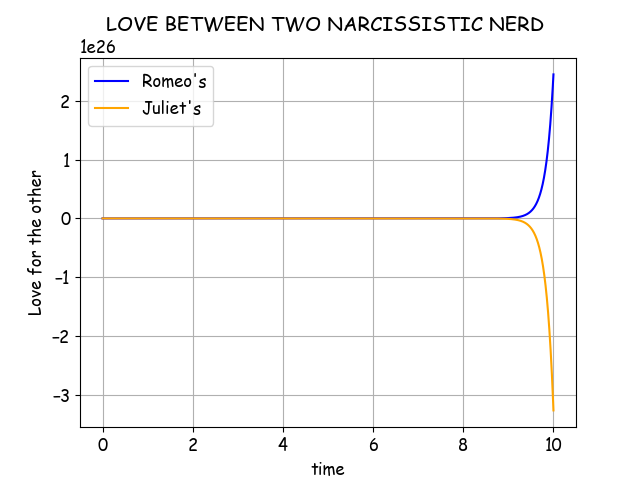
\includegraphics[width=100mm]{image/bt2/plot2.1.png}
    \caption{VD2.1 - The plot of the love between two Narcissistic Nerd }
\end{figure}

\textbf{Dạng Phase portrait: } Saddle
\begin{figure}[!htbp]
    \centering
    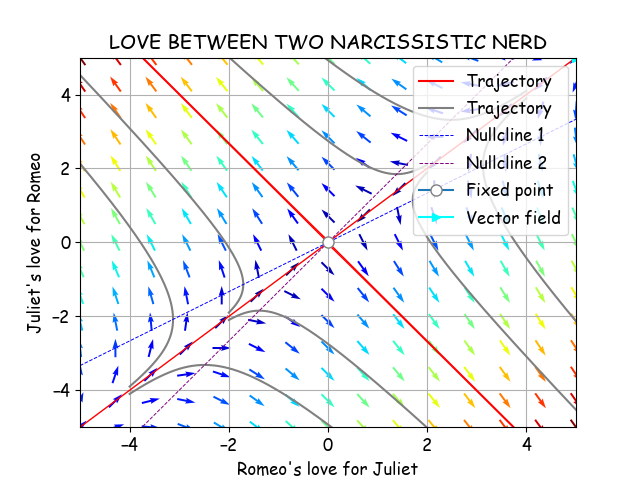
\includegraphics[width=100mm]{image/bt2/pp2.1.png}
    \caption{VD2.1 - The phase portrait of the love between two Narcissistic Nerd}
\end{figure}
\pagebreak
\begin{figure}[!htbp]
    \centering
    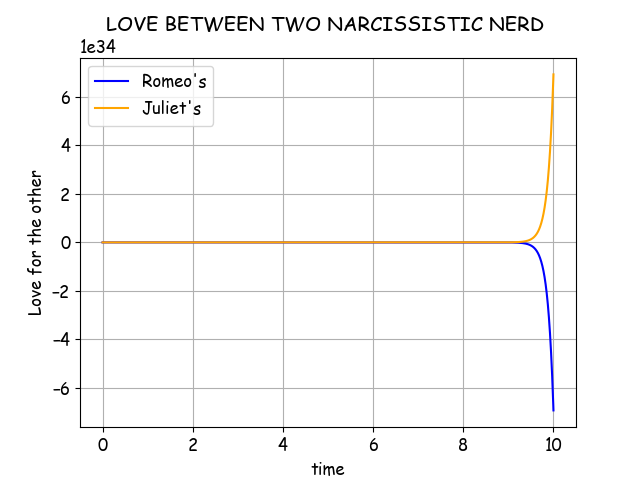
\includegraphics[width=100mm]{image/bt2/plot2.2.png}
    \caption{VD2.2 - The plot of the love between two Narcissistic Nerd}
\end{figure}
\begin{figure}[!htbp]
    \centering
    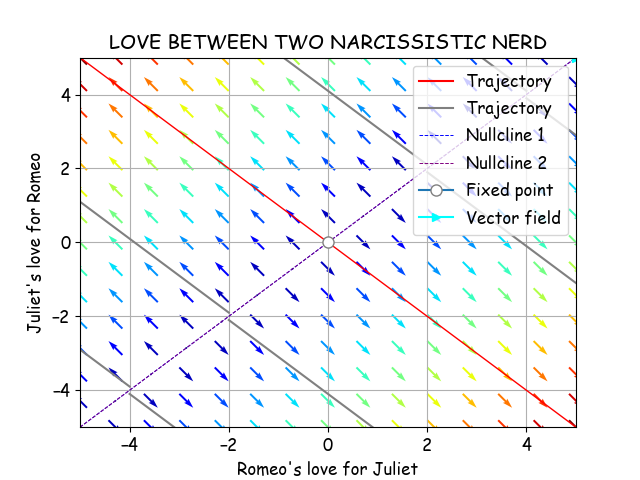
\includegraphics[width=100mm]{image/bt2/pp2.2.png}
    \caption{VD2.2 - The phase portrait of the love between two Narcissistic Nerd}
\end{figure}

\textbf{Dạng Phase portrait: } Unstable Saddle-Node
\pagebreak
%%%%%%%%%%%%%%%%%%33333333333%%%%%%%%%%%%%%%%%%%%%%%%
%%%%%%%%%%%%%%%%%%%%%%%%%%%%%%%%%%%%%%%%%%%%%%%%%%%%%
\begin{tcbdoublebox}[title={3. Cautious Lover and Cautious Lover}]
\mdseries .\\
\bfseries Ví dụ 1: \\
\textcolor{blue}{$$\left\{\begin{matrix}
\dot{R} =  -3R + 4J \\ 
\dot{J} =  2R-5J\\ 
R(0)= - \frac{-3}{4}, J(0)=\frac{5}{4}
\end{matrix}\right.$$}\\
\mdseries Ma trận $\color{blue}A=\begin{pmatrix}
-3 & 4\\ 
2 & -5
\end{pmatrix}$ có hai trị riêng là 
$\color{blue}\lambda_{1}=-1;\ \lambda_{2}=-7$
, lần lượt tương ứng với các vecto riêng:
$\color{blue}v_{1} = (2;\ 1)^{T};\ v_{2}=(-1;\ 1)^{T}$\\Áp dụng công thức bài tập 1, nghiệm của hệ phương trình là:
$$R(t)=\frac{{\mathrm{e}}^{-t}}{3}-\frac{13\,{\mathrm{e}}^{-7\,t}}{12} $$
$$J(t)=\frac{{\mathrm{e}}^{-t}}{6}+\frac{13\,{\mathrm{e}}^{-7\,t}}{12}$$
\\
\bfseries Ví dụ 2:\\
\textcolor{blue}{$$\left\{\begin{matrix}
\dot{R} =  -\frac{5}{2}R + \frac{5}{2}J \\ 
\dot{J} =  3R -3J\\ 
R(0)= \frac{4}{5}, J(0)=\frac{9}{5}
\end{matrix}\right.$$}
\mdseries Ma trận $\color{blue}A=\begin{pmatrix}
-\frac{5}{2} & \frac{5}{2}\\ 
3 & -3
\end{pmatrix}$ có hai trị riêng là 
$\color{blue}\lambda_{1}=0;\ \lambda_{2}=-\frac{11}{2}$
, lần lượt tương ứng với các vecto riêng:
$\color{blue}v_{1} = (1;\ 1)^{T};\ v_{2}=(-\frac{5}{6};\ 1)^{T}$\\Áp dụng công thức bài tập 1, nghiệm của hệ phương trình là:
$$R(t)=\frac{69}{55}-\frac{5\,{\mathrm{e}}^{-\frac{11\,t}{2}}}{11}$$
$$J(t)=\frac{6\,{\mathrm{e}}^{-\frac{11\,t}{2}}}{11}+\frac{69}{55}$$

\textbf{Nhận xét: } Trong trường hợp này, cả Romeo và Juliet đều là Cautious Lover. Theo định nghĩa, Cautious Lover có xu hướng không bị khuyến khích bởi tình cảm của mình và phản ứng với tình cảm của đối phương. Trong \textbf{Ví dụ 1}, ta thấy rằng, ban đầu có người thích có người ghét đối phương, vì vậy theo thời gian thì tình cảm của 2 người sẽ dần tiến tới 0, còn trong \textbf{Ví dụ 2} sẽ tiến tới một hằng số nhất định bởi ban đầu cả hai đều có tình ý với đối phương.

Hai cặp \textbf{đồ thị plot và phase portrait} dưới đây sẽ mô tả cho điều này!
\end{tcbdoublebox}
\pagebreak
\begin{figure}[!htbp]
    \centering
    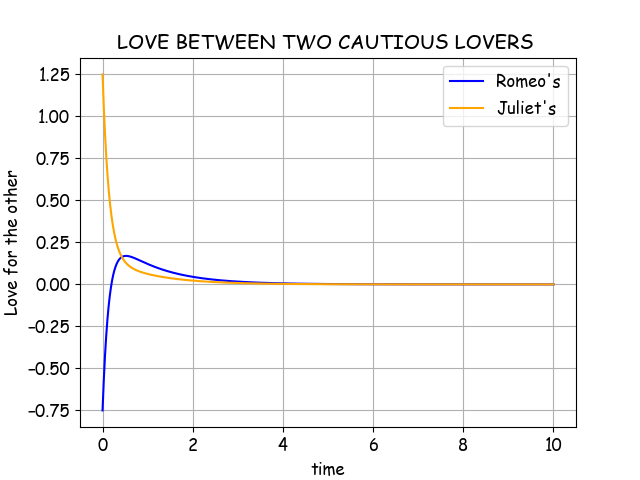
\includegraphics[width=100mm]{image/bt2/plot3.1.png}
    \caption{VD3.1 - The plot of the love between two Cautious Lovers }
\end{figure}
\begin{figure}[!htbp]
    \centering
    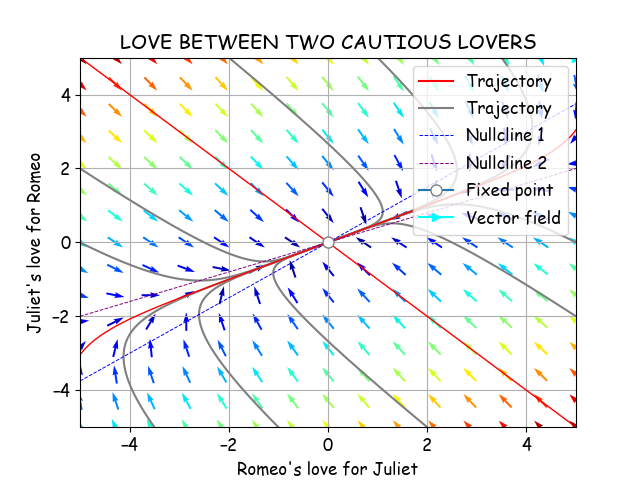
\includegraphics[width=100mm]{image/bt2/pp3.1.png}
    \caption{VD3.1 - The phase portrait of the love between two Cautious Lovers}
\end{figure}

\textbf{Dạng Phase portrait: } Nodal Sink
\pagebreak
\begin{figure}[!htbp]
    \centering
    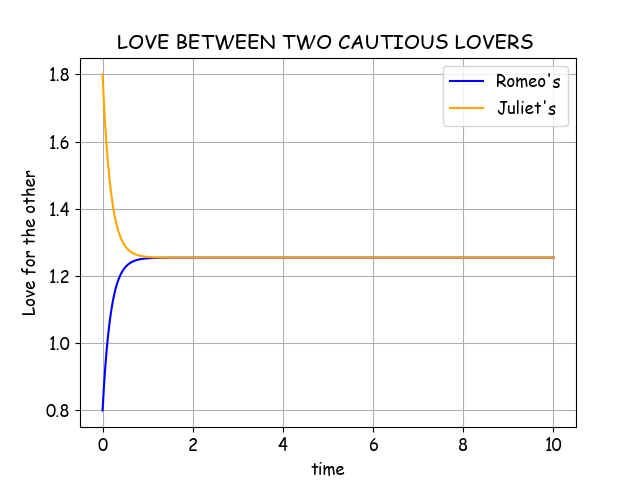
\includegraphics[width=100mm]{image/bt2/plot3.2.png}
    \caption{VD3.2 - The plot of the love between two Cautious Lovers}
\end{figure}
\begin{figure}[!htbp]
    \centering
    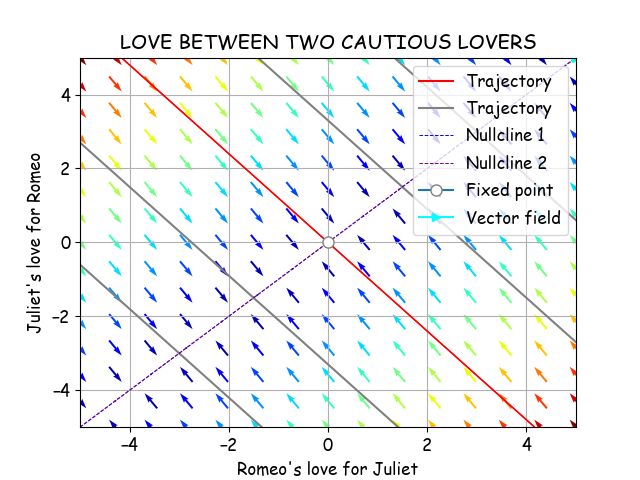
\includegraphics[width=100mm]{image/bt2/pp3.2.png}
    \caption{VD3.2 - The phase portrait of the love between two Cautious Lovers}
\end{figure}

\textbf{Dạng Phase portrait: } Stable Saddle-Node
\pagebreak
%%%%%%%%%%%%%%%%%%44444444444%%%%%%%%%%%%%%%%%%%%%%%%
%%%%%%%%%%%%%%%%%%%%%%%%%%%%%%%%%%%%%%%%%%%%%%%%%%%%%
\begin{tcbdoublebox}[title={4. Hermit and Hermit}]
\mdseries .\\
\bfseries Ví dụ 1: \\
\textcolor{blue}{$$\left\{\begin{matrix}
\dot{R} =  -3R -5J \\ 
\dot{J} =  -4R-2J\\ 
R(0)= -\frac{1}{6}, J(0)=\frac{3}{2}
\end{matrix}\right.$$}\\
\mdseries Ma trận $\color{blue}A=\begin{pmatrix}
-3 & -5\\ 
-4 & -2
\end{pmatrix}$ có hai trị riêng là 
$\color{blue}\lambda_{1}=-7;\ \lambda_{2}=2$
, lần lượt tương ứng với các vecto riêng:
$\color{blue}v_{1} = (5;\ 4)^{T};\ v_{2}=(-1;\ 1)^{T}$\\Áp dụng công thức bài tập 1, nghiệm của hệ phương trình là:
$$R(t)=\frac{20\,{\mathrm{e}}^{-7\,t}}{27}-\frac{49\,{\mathrm{e}}^{2\,t}}{54} $$
$$J(t)=\frac{49\,{\mathrm{e}}^{2\,t}}{54}+\frac{16\,{\mathrm{e}}^{-7\,t}}{27}$$
\\
\bfseries Ví dụ 2:\\
\textcolor{blue}{$$\left\{\begin{matrix}
\dot{R} =  -7R -9J \\ 
\dot{J} =  -4R -11J\\ 
R(0)= 3, J(0)=5
\end{matrix}\right.$$}
\mdseries Ma trận $\color{blue}A=\begin{pmatrix}
-7 & -9\\ 
-4 & -11
\end{pmatrix}$ có hai trị riêng là 
$\color{blue}\lambda_{1}=-9+2\sqrt{10};\ \lambda_{2}=-9-2\sqrt{10}$
, lần lượt tương ứng với các vecto riêng:
$\color{blue}v_{1} = (-1-\sqrt{10};\ 2)^{T};\ v_{2}=(-1+\sqrt{10};\ 2)^{T}$\\Áp dụng công thức bài tập 1, nghiệm của hệ phương trình là:
$$R(t)={\mathrm{e}}^{t\,\left(2\,\sqrt{10}-9\right)}\,\left(\frac{\sqrt{10}}{2}+\frac{1}{2}\right)\,\left(\frac{11\,\sqrt{10}}{20}-\frac{5}{2}\right)+\frac{\sqrt{10}\,{\mathrm{e}}^{-t\,\left(2\,\sqrt{10}+9\right)}\,\left(\frac{\sqrt{10}}{2}-\frac{1}{2}\right)\,\left(5\,\sqrt{10}+11\right)}{20}$$
$$J(t)=\frac{\sqrt{10}\,{\mathrm{e}}^{-t\,\left(2\,\sqrt{10}+9\right)}\,\left(5\,\sqrt{10}+11\right)}{20}-{\mathrm{e}}^{t\,\left(2\,\sqrt{10}-9\right)}\,\left(\frac{11\,\sqrt{10}}{20}-\frac{5}{2}\right)$$

\textbf{Nhận xét: } Trong trường hợp này, cả Romeo và Juliet đều là Hermit. Theo định nghĩa, Hermit sẽ có xu hướng không bị khuyến khích bởi tình cảm của bản thân
cũng như đối phương. Trong \textbf{Ví dụ 1}, , còn trong \textbf{Ví dụ 2} ban đầu ta thấy cả 2 người đều thích nhau, tuy nhiên vì họ là Hermit nên
ban đầu tình cảm của họ giảm dần và giữ nguyên khi thời gian tăng lên.

Hai cặp \textbf{đồ thị plot và phase portrait} dưới đây sẽ mô tả cho điều này!
\end{tcbdoublebox}
\pagebreak
\begin{figure}[!htbp]
    \centering
    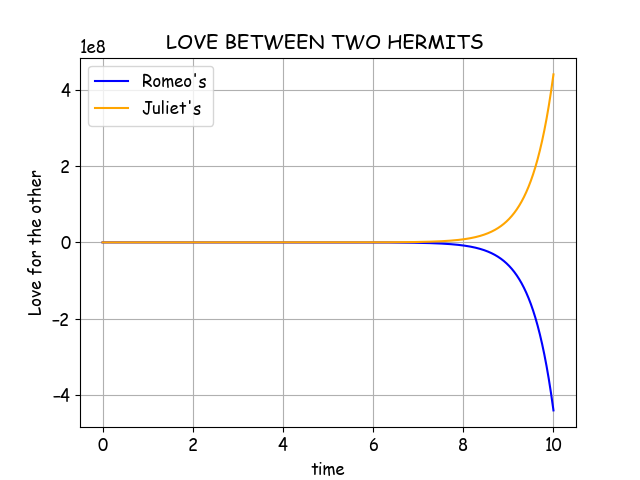
\includegraphics[width=100mm]{image/bt2/plot4.1.png}
    \caption{VD4.1 - The plot of the love between two Hermits }
\end{figure}
\begin{figure}[!htbp]
    \centering
    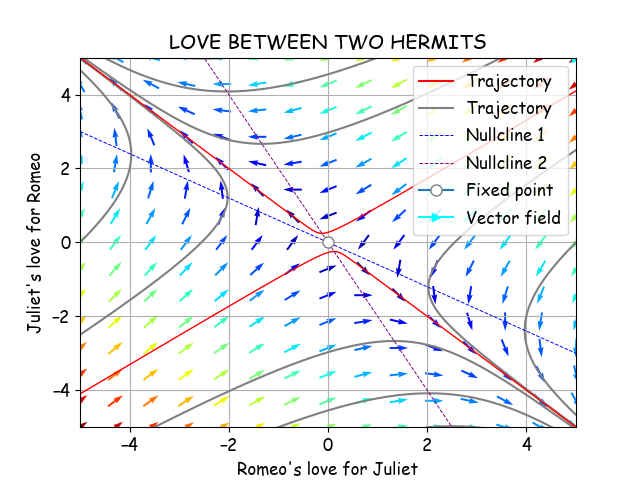
\includegraphics[width=100mm]{image/bt2/pp4.1.png}
    \caption{VD4.1 - The phase portrait of the love between two Hermits}
\end{figure}

\textbf{Dạng Phase portrait: } Saddle
\pagebreak
\begin{figure}[!htbp]
    \centering
    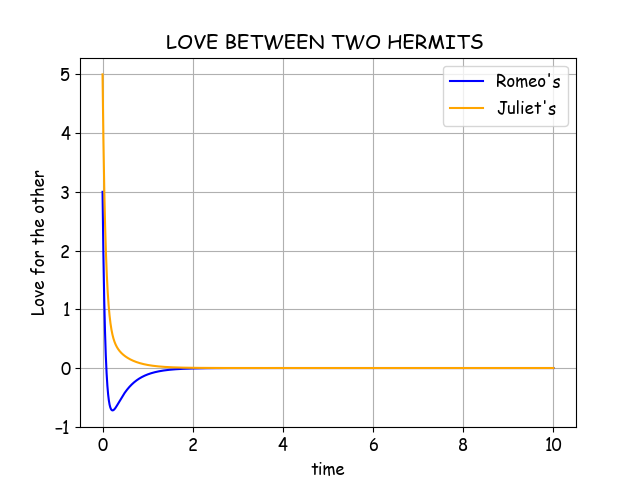
\includegraphics[width=100mm]{image/bt2/plot4.2.png}
    \caption{VD4.2 - The plot of the love between two Hermits}
\end{figure}
\begin{figure}[!htbp]
    \centering
    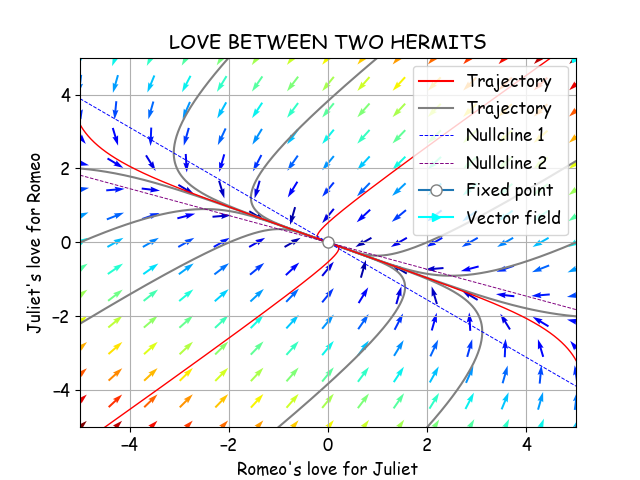
\includegraphics[width=100mm]{image/bt2/pp4.2.png}
    \caption{VD4.2 - The phase portrait of the love between two Hermits}
\end{figure}

\textbf{Dạng Phase portrait: } Spiral Sink
\pagebreak
%%%%%%%%%%%%%%%%%%55555555555%%%%%%%%%%%%%%%%%%%%%%%%
%%%%%%%%%%%%%%%%%%%%%%%%%%%%%%%%%%%%%%%%%%%%%%%%%%%%%
\begin{tcbdoublebox}[title={5. Eager Beaver and Narcissistic Nerd}]
\mdseries .\\
\bfseries Ví dụ 1: \\
\textcolor{blue}{$$\left\{\begin{matrix}
\dot{R} =  1R +6J \\ 
\dot{J} =  -3R+7J\\ 
R(0)= -3, J(0)=5
\end{matrix}\right.$$}\\
\mdseries Ma trận $\color{blue}A=\begin{pmatrix}
1 & 6\\ 
-3 & 7
\end{pmatrix}$ có hai trị riêng là 
$\color{blue}\lambda_{1}=4+3i;\ \lambda_{2}=4-3i$
, lần lượt tương ứng với các vecto riêng:
$\color{blue}v_{1} = (1-i;\ 1)^{T};\ v_{2}=(1+i;\ 1)^{T}$\\Áp dụng công thức bài tập 1, nghiệm của hệ phương trình là:
$$R(t)=3\,\cos\left(3\,t\right)\,{\mathrm{e}}^{4\,t}+7\,\sin\left(3\,t\right)\,{\mathrm{e}}^{4\,t} $$
$$J(t)=5\,\cos\left(3\,t\right)\,{\mathrm{e}}^{4\,t}+2\,\sin\left(3\,t\right)\,{\mathrm{e}}^{4\,t}$$
\\
\bfseries Ví dụ 2:\\
\textcolor{blue}{$$\left\{\begin{matrix}
\dot{R} = 5R -2J \\ 
\dot{J} =  2R +1J\\ 
R(0)= \frac{9}{4}, J(0)=\frac{5}{4}
\end{matrix}\right.$$}
\mdseries Ma trận $\color{blue}A=\begin{pmatrix}
5 & -2\\ 
2 & 1
\end{pmatrix}$ có trị riêng bội 2 là 
$\color{blue}\lambda_{1}=\lambda_{2}=3$ tương ứng với vecto riêng:
$\color{blue}v_{1} = v_{2}=(1;\ 1)^{T}$\\Áp dụng công thức bài tập 1, nghiệm của hệ phương trình là:
$$R(t)=\frac{9\,{\mathrm{e}}^{3\,t}}{4}+2\,t\,{\mathrm{e}}^{3\,t}$$
$$J(t)=\frac{5\,{\mathrm{e}}^{3\,t}}{4}+2\,t\,{\mathrm{e}}^{3\,t}$$

\end{tcbdoublebox}
\pagebreak
\begin{figure}[!htbp]
    \centering
    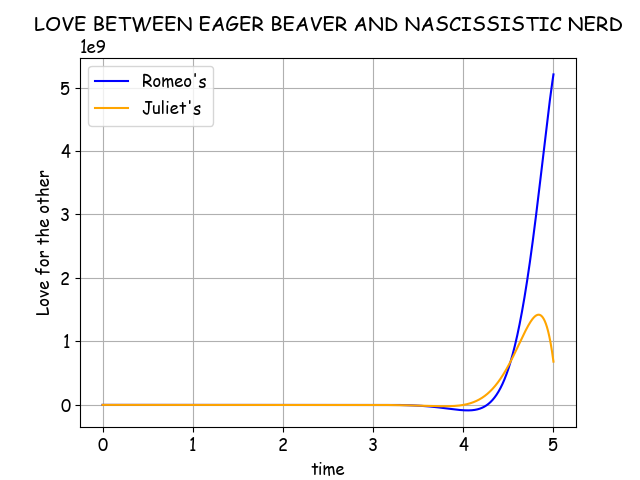
\includegraphics[width=100mm]{image/bt2/plot5.1.png}
    \caption{VD5.1 - The plot of the love between Eager Beaver and Narcissistic Nerd}
\end{figure}
\begin{figure}[!htbp]
    \centering
    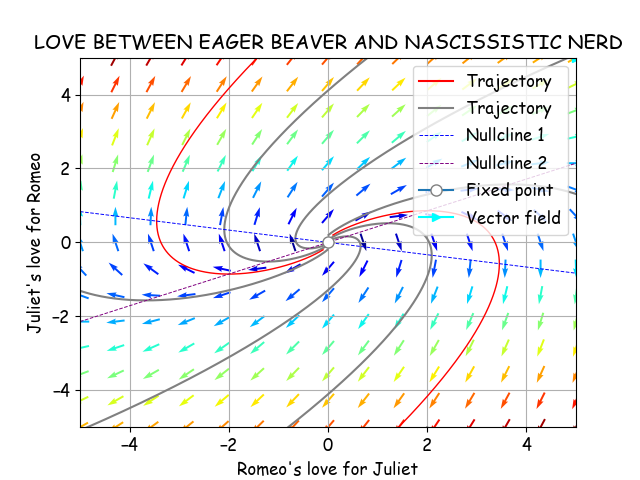
\includegraphics[width=100mm]{image/bt2/pp5.1.png}
    \caption{VD5.1 - The phase portrait of the love between Eager Beaver and Narcissistic Nerd}
\end{figure}

\textbf{Dạng Phase portrait: } Spiral Source
\pagebreak
\begin{figure}[!htbp]
    \centering
    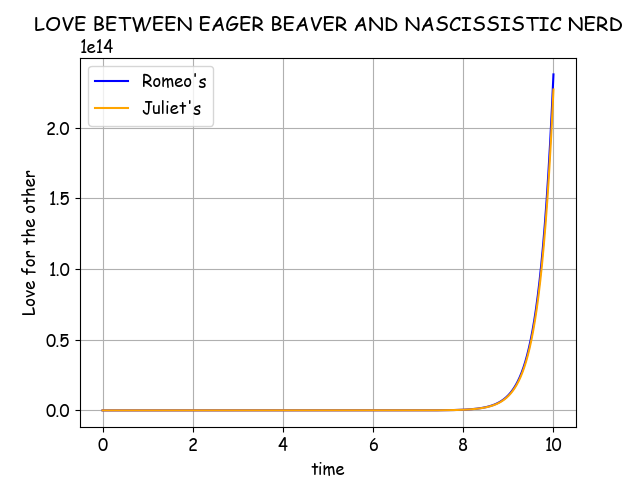
\includegraphics[width=100mm]{image/bt2/plot5.2.png}
    \caption{VD5.2 - The plot of the love between Eager Beaver and Narcissistic Nerd}
\end{figure}
\begin{figure}[!htbp]
    \centering
    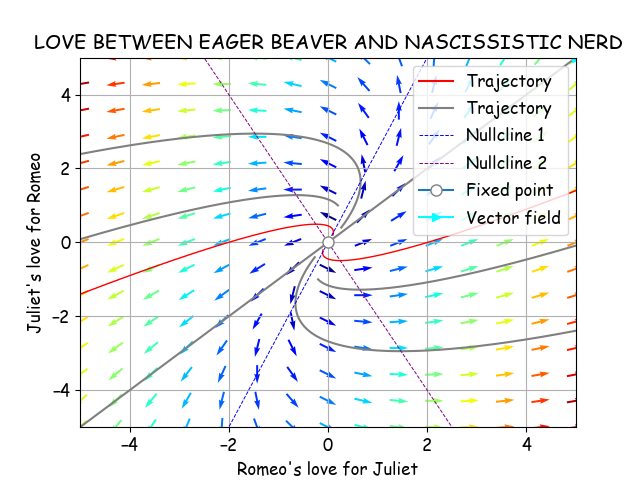
\includegraphics[width=100mm]{image/bt2/pp5.2.png}
    \caption{VD5.2 - The phase portrait of the love between Eager Beaver and Narcissistic Nerd}
\end{figure}

\textbf{Dạng Phase portrait: } Degenerate Nodal Source
\pagebreak
%%%%%%%%%%%%%%%%%%666666666666%%%%%%%%%%%%%%%%%%%%%%%%
%%%%%%%%%%%%%%%%%%%%%%%%%%%%%%%%%%%%%%%%%%%%%%%%%%%%%
\begin{tcbdoublebox}[title={6. Eager Beaver and Cautious Lover}]
\mdseries .\\
\bfseries Ví dụ 1: \\
\textcolor{blue}{$$\left\{\begin{matrix}
\dot{R} =  3R +J \\ 
\dot{J} =  2R-3J\\ 
R(0)= 2, J(0)=0
\end{matrix}\right.$$}\\
\mdseries Ma trận $\color{blue}A=\begin{pmatrix}
-3 & -5\\ 
-4 & -2
\end{pmatrix}$ có hai trị riêng là 
$\color{blue}\lambda_{1}=-\sqrt{11};\ \lambda_{2}=\sqrt{11}$
, lần lượt tương ứng với các vecto riêng:
$\color{blue}v_{1} = (3-\sqrt{11};\ 2)^{T};\ v_{2}=(3+\sqrt{11};\ 2)^{T}$\\Áp dụng công thức bài tập 1, nghiệm của hệ phương trình là:
$$R(t)=\frac{2\,\sqrt{11}\,{\mathrm{e}}^{\sqrt{11}\,t}\,\left(\frac{\sqrt{11}}{2}+\frac{3}{2}\right)}{11}+\frac{2\,\sqrt{11}\,{\mathrm{e}}^{-\sqrt{11}\,t}\,\left(\frac{\sqrt{11}}{2}-\frac{3}{2}\right)}{11}$$
$$J(t)=\frac{2\,\sqrt{11}\,{\mathrm{e}}^{\sqrt{11}\,t}}{11}-\frac{2\,\sqrt{11}\,{\mathrm{e}}^{-\sqrt{11}\,t}}{11}$$
\\
\bfseries Ví dụ 2:\\
\textcolor{blue}{$$\left\{\begin{matrix}
\dot{R} = -2R +J \\ 
\dot{J} =  5R +2J\\ 
R(0)= -4, J(0)=2
\end{matrix}\right.$$}
\mdseries Ma trận $\color{blue}A=\begin{pmatrix}
-2 & 1\\ 
5 & 2
\end{pmatrix}$ có hai trị riêng là 
$\color{blue}\lambda_{1}=3;\ \lambda_{2}=-3$
, lần lượt tương ứng với các vecto riêng:
$\color{blue}v_{1} = (1;\ 5)^{T};\ v_{2}=(-1;\ 1)^{T}$\\Áp dụng công thức bài tập 1, nghiệm của hệ phương trình là:
$$R(t)=-\frac{11\,{\mathrm{e}}^{-3\,t}}{3}-\frac{{\mathrm{e}}^{3\,t}}{3}$$
$$J(t)=\frac{11\,{\mathrm{e}}^{-3\,t}}{3}-\frac{5\,{\mathrm{e}}^{3\,t}}{3}$$

\end{tcbdoublebox}
\pagebreak
\begin{figure}[!htbp]
    \centering
    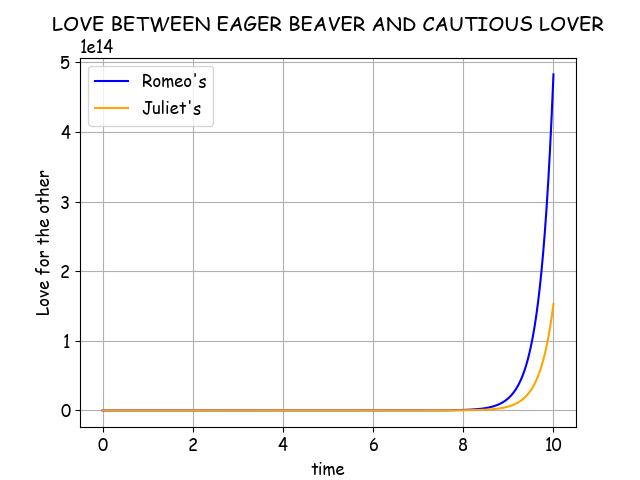
\includegraphics[width=100mm]{image/bt2/plot6.1.png}
    \caption{VD6.1 - The plot of the love between Eager Beaver and Cautious Lover}
\end{figure}
\begin{figure}[!htbp]
    \centering
    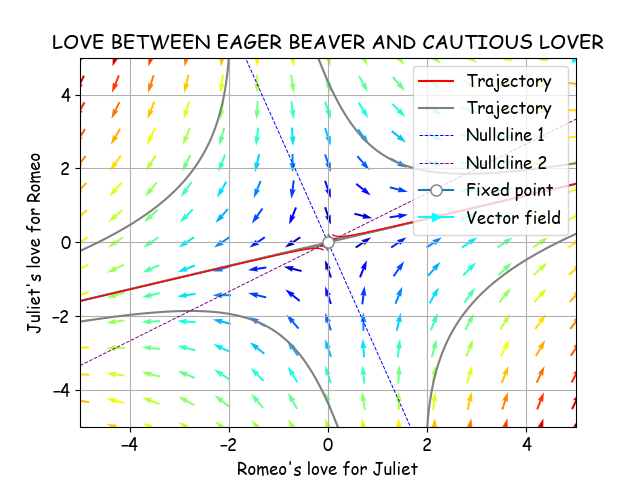
\includegraphics[width=100mm]{image/bt2/pp6.1.png}
    \caption{VD6.1 - The phase portrait of the love between Eager Beaver and Cautious Lover}
\end{figure}

\textbf{Dạng Phase portrait: } Saddle
\pagebreak
\begin{figure}[!htbp]
    \centering
    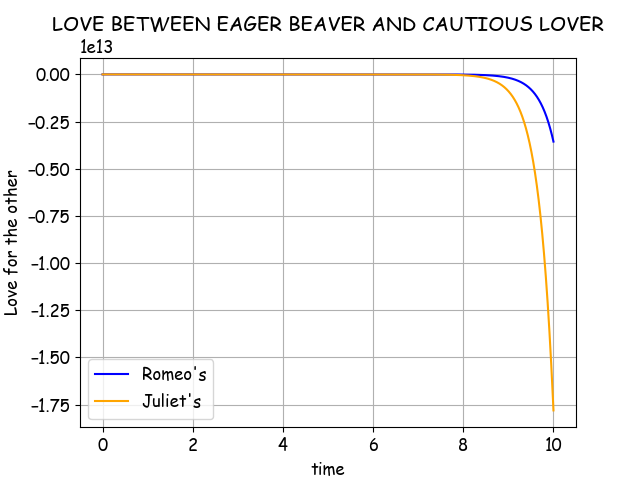
\includegraphics[width=100mm]{image/bt2/plot6.2.png}
    \caption{VD6.2 - The plot of the love between Eager Beaver and Cautious Lover}
\end{figure}
\begin{figure}[!htbp]
    \centering
    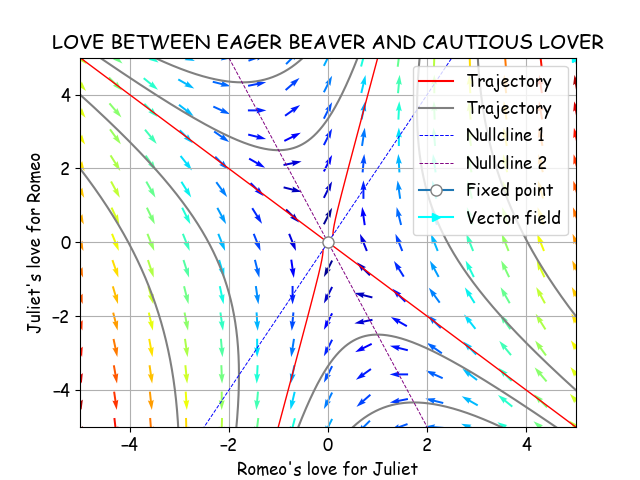
\includegraphics[width=100mm]{image/bt2/pp6.2.png}
    \caption{VD6.2 - The phase portrait of the love between Eager Beaver and Cautious Lover}
\end{figure}

\textbf{Dạng Phase portrait: } Saddle
\pagebreak
%%%%%%%%%%%%%%%%%%77777777777%%%%%%%%%%%%%%%%%%%%%%%%
%%%%%%%%%%%%%%%%%%%%%%%%%%%%%%%%%%%%%%%%%%%%%%%%%%%%%
\begin{tcbdoublebox}[title={7. Eager Beaver and Hermit}]
\mdseries .\\
\bfseries Ví dụ 1: \\
\textcolor{blue}{$$\left\{\begin{matrix}
\dot{R} =  5R +10J \\ 
\dot{J} =  -5R-5J\\ 
R(0)= -\frac{7}{2}, J(0)=\frac{3}{2}
\end{matrix}\right.$$}\\
\mdseries Ma trận $\color{blue}A=\begin{pmatrix}
5 & 10\\ 
-5 & -5
\end{pmatrix}$ có hai trị riêng là 
$\color{blue}\lambda_{1}=5i;\ \lambda_{2}=-5i$
, lần lượt tương ứng với các vecto riêng:
$\color{blue}v_{1} = (-1-i;\ 1)^{T};\ v_{2}=(-1+i;\ 1)^{T}$\\Áp dụng công thức bài tập 1, nghiệm của hệ phương trình là:
$$R(t)=-\frac{7\,\cos\left(5\,t\right)}{2}-\frac{\sin\left(5\,t\right)}{2}$$
$$J(t)=\frac{3\,\cos\left(5\,t\right)}{2}+2\,\sin\left(5\,t\right)$$
\\
\bfseries Ví dụ 2:\\
\textcolor{blue}{$$\left\{\begin{matrix}
\dot{R} = -3R -2J \\ 
\dot{J} =  4R +J\\ 
R(0)= -\frac{12}{5}, J(0)=\frac{9}{4}
\end{matrix}\right.$$}
\mdseries Ma trận $\color{blue}A=\begin{pmatrix}
-3 & -2\\ 
4 & 1
\end{pmatrix}$ có hai trị riêng là 
$\color{blue}\lambda_{1}=-1+2i;\ \lambda_{2}=-1-2i$
, lần lượt tương ứng với các vecto riêng:
$\color{blue}v_{1} = (-1+i;\ 2)^{T};\ v_{2}=(-1-i;\ 2)^{T}$\\Áp dụng công thức bài tập 1, nghiệm của hệ phương trình là:
$$R(t)=\frac{3\,\sin\left(2\,t\right)\,{\mathrm{e}}^{-t}}{20}-\frac{12\,\cos\left(2\,t\right)\,{\mathrm{e}}^{-t}}{5}$$
$$J(t)=\frac{9\,\cos\left(2\,t\right)\,{\mathrm{e}}^{-t}}{4}-\frac{51\,\sin\left(2\,t\right)\,{\mathrm{e}}^{-t}}{20}$$

\end{tcbdoublebox}
\pagebreak
\begin{figure}[!htbp]
    \centering
    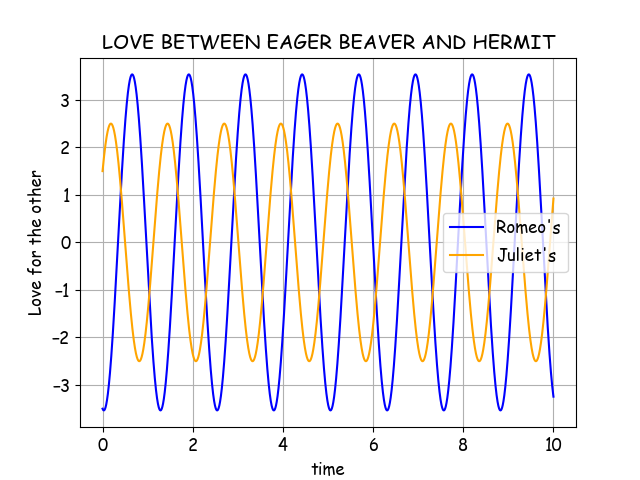
\includegraphics[width=100mm]{image/bt2/plot7.1.png}
    \caption{VD7.1 - The plot of the love between Eager Beaver and Hermit}
\end{figure}
\begin{figure}[!htbp]
    \centering
    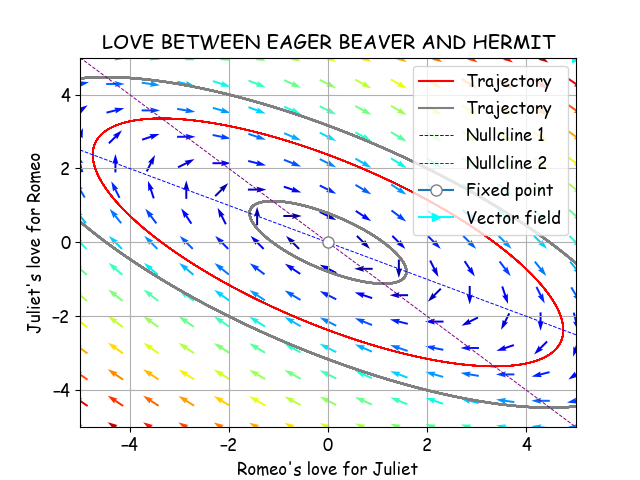
\includegraphics[width=100mm]{image/bt2/pp7.1.png}
    \caption{VD7.1 - The phase portrait of the love between Eager Beaver and Hermit}
\end{figure}

\textbf{Dạng Phase portrait: } Center
\pagebreak
\begin{figure}[!htbp]
    \centering
    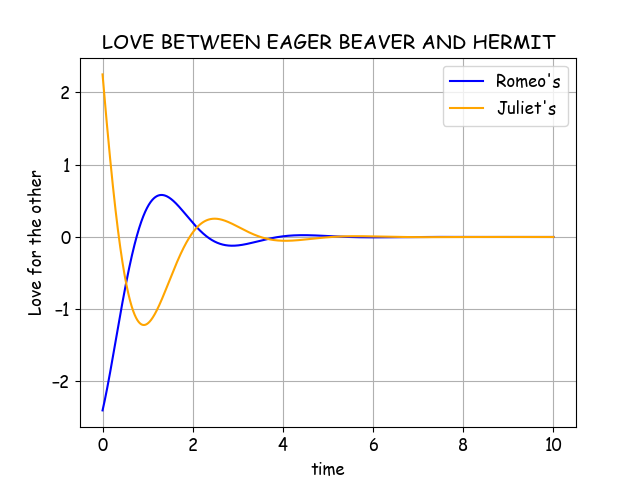
\includegraphics[width=100mm]{image/bt2/plot7.2.png}
    \caption{VD7.2 - The plot of the love between Eager Beaver and Hermit}
\end{figure}
\begin{figure}[!htbp]
    \centering
    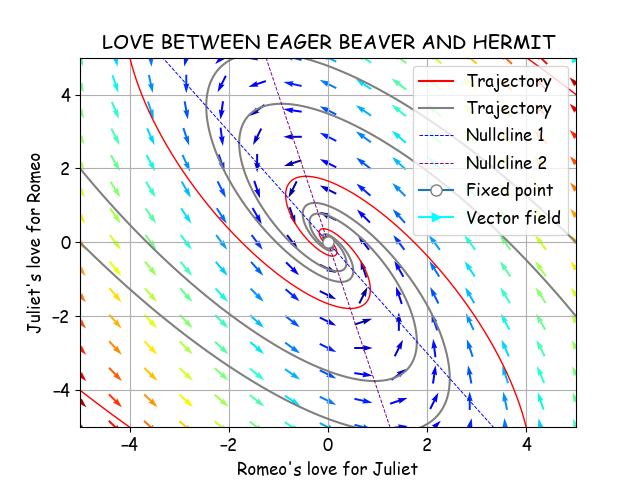
\includegraphics[width=100mm]{image/bt2/pp7.2.png}
    \caption{VD7.2 - The phase portrait of the love between Eager Beaver and Hermit}
\end{figure}

\textbf{Dạng Phase portrait: } Spiral Sink
\pagebreak
%%%%%%%%%%%%%%%%%%888888888888%%%%%%%%%%%%%%%%%%%%%%%%
%%%%%%%%%%%%%%%%%%%%%%%%%%%%%%%%%%%%%%%%%%%%%%%%%%%%%
\begin{tcbdoublebox}[title={8. Narcissistic Nerd and Cautious Lover}]
\mdseries .\\
\bfseries Ví dụ 1: \\
\textcolor{blue}{$$\left\{\begin{matrix}
\dot{R} =  2R -4J \\ 
\dot{J} =  R-2J\\ 
R(0)= -\frac{9}{2}, J(0)=3
\end{matrix}\right.$$}\\
\mdseries Ma trận $\color{blue}A=\begin{pmatrix}
2 & -4\\ 
1 & -2
\end{pmatrix}$ có trị riêng bội 2 là 
$\color{blue}\lambda_{1}=\lambda_{2}=0$ tương ứng với các vecto riêng:
$\color{blue}v = (2;\ 1)^{T};$\\Áp dụng công thức bài tập 1, nghiệm của hệ phương trình là:
$$R(t)=-21\,t-\frac{9}{2}$$
$$J(t)=3-\frac{21\,t}{2}$$
\\
\bfseries Ví dụ 2:\\
\textcolor{blue}{$$\left\{\begin{matrix}
\dot{R} = 3R -4J \\ 
\dot{J} =  5R -J\\ 
R(0)= -2, J(0)=-3
\end{matrix}\right.$$}
\mdseries Ma trận $\color{blue}A=\begin{pmatrix}
3 & -4\\ 
5 & -1
\end{pmatrix}$ có hai trị riêng là 
$\color{blue}\lambda_{1}=1+4i;\ \lambda_{2}=1-4i$
, lần lượt tương ứng với các vecto riêng:
$\color{blue}v_{1} = (2+4i;\ 5)^{T};\ v_{2}=(2-4i;\ 5)^{T}$\\Áp dụng công thức bài tập 1, nghiệm của hệ phương trình là:
$$R(t)=2\,\sin\left(4\,t\right)\,{\mathrm{e}}^t-2\,\cos\left(4\,t\right)\,{\mathrm{e}}^t$$
$$J(t)=-3\,\cos\left(4\,t\right)\,{\mathrm{e}}^t-\sin\left(4\,t\right)\,{\mathrm{e}}^t$$

\end{tcbdoublebox}
\pagebreak
\begin{figure}[!htbp]
    \centering
    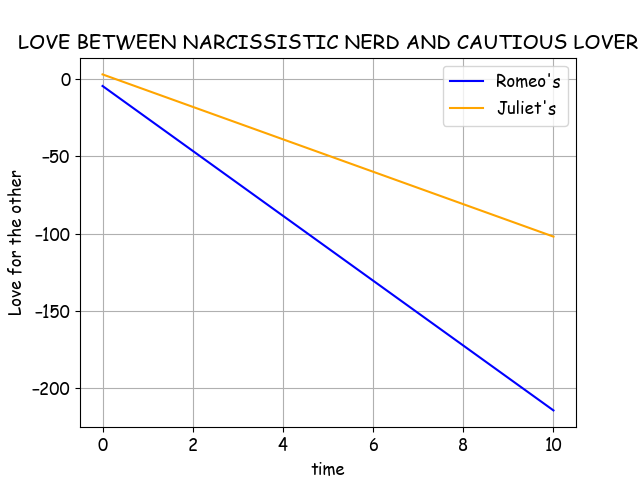
\includegraphics[width=100mm]{image/bt2/plot8.1.png}
    \caption{VD8.1 - The plot of the love between Narcissistic Nerd and Cautious Lover}
\end{figure}
\begin{figure}[!htbp]
    \centering
    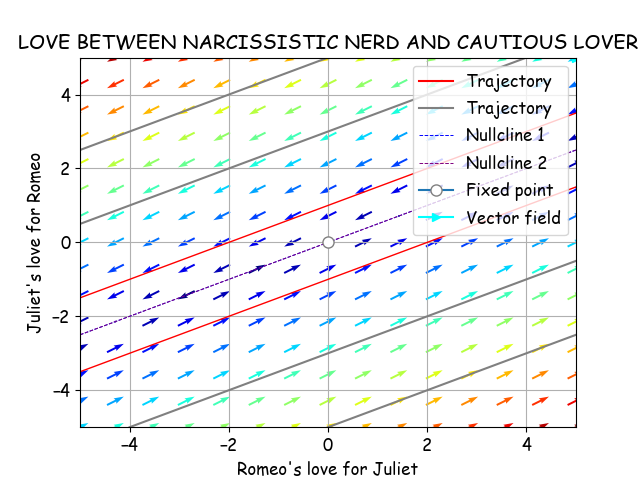
\includegraphics[width=100mm]{image/bt2/pp8.1.png}
    \caption{VD8.1 - The phase portrait of the love between Narcissistic Nerd and Cautious Lover}
\end{figure}

\textbf{Dạng Phase portrait: } Pure Shear
\pagebreak
\begin{figure}[!htbp]
    \centering
    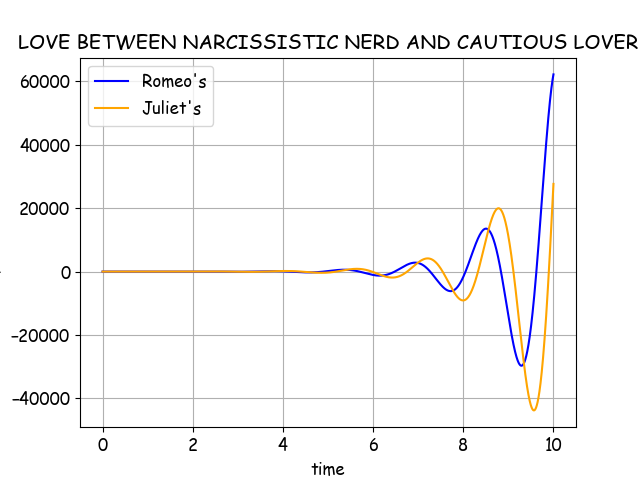
\includegraphics[width=100mm]{image/bt2/plot8.2.png}
    \caption{VD8.2 - The plot of the love between Narcissistic Nerd and Cautious Lover}
\end{figure}
\begin{figure}[!htbp]
    \centering
    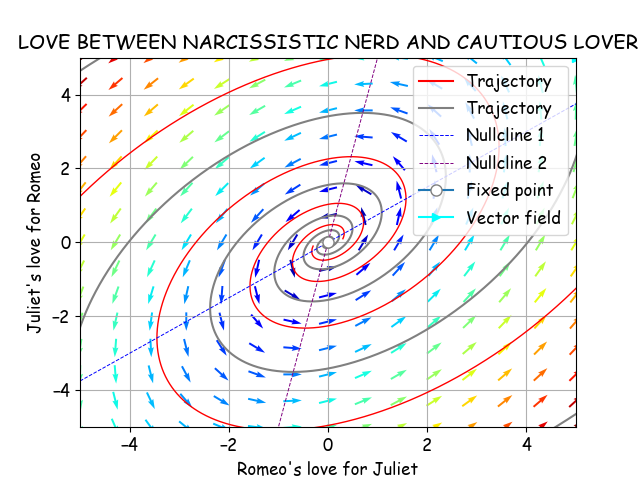
\includegraphics[width=100mm]{image/bt2/pp8.2.png}
    \caption{VD8.2 - The phase portrait of the love between Narcissistic Nerd and Cautious Lover}
\end{figure}

\textbf{Dạng Phase portrait: } Spiral Source
\pagebreak
%%%%%%%%%%%%%%%%%%99999999999%%%%%%%%%%%%%%%%%%%%%%%%
%%%%%%%%%%%%%%%%%%%%%%%%%%%%%%%%%%%%%%%%%%%%%%%%%%%%%
\begin{tcbdoublebox}[title={9. Narcissistic Nerd and Hermit}]
\mdseries .\\
\bfseries Ví dụ 1: \\
\textcolor{blue}{$$\left\{\begin{matrix}
\dot{R} =  3R -2J \\ 
\dot{J} =  -3R-2J\\ 
R(0)= 4, J(0)=4
\end{matrix}\right.$$}\\
\mdseries Ma trận $\color{blue}A=\begin{pmatrix}
3 & -2\\ 
-3 & -2
\end{pmatrix}$ có hai trị riêng là 
$\color{blue}\lambda_{1}=4;\ \lambda_{2}=-3$
, lần lượt tương ứng với các vecto riêng:
$\color{blue}v_{1} = (-2;\ 1)^{T};\ v_{2}=(1;\ 3)^{T}$\\Áp dụng công thức bài tập 1, nghiệm của hệ phương trình là:
$$R(t)=\frac{12\,{\mathrm{e}}^{-3\,t}}{7}+\frac{16\,{\mathrm{e}}^{4\,t}}{7}$$
$$J(t)=\frac{36\,{\mathrm{e}}^{-3\,t}}{7}-\frac{8\,{\mathrm{e}}^{4\,t}}{7}$$
\\
\bfseries Ví dụ 2:\\
\textcolor{blue}{$$\left\{\begin{matrix}
\dot{R} = 2R -1J \\ 
\dot{J} =  -4R -2J\\ 
R(0)= -2, J(0)=1
\end{matrix}\right.$$}
\mdseries Ma trận $\color{blue}A=\begin{pmatrix}
2 & -1\\ 
-4 & -2
\end{pmatrix}$ có hai trị riêng là 
$\color{blue}\lambda_{1}=2\sqrt{2};\ \lambda_{2}=-2\sqrt{2}$
, lần lượt tương ứng với các vecto riêng:
$\color{blue}v_{1} = (-1-\sqrt{2};\ 2)^{T};\ v_{2}=(-1+\sqrt{2};\ 2)^{T}$\\Áp dụng công thức bài tập 1, nghiệm của hệ phương trình là:
$$R(t)=\frac{\sqrt{8}\,{\mathrm{e}}^{-\sqrt{8}\,t}\,\left(\frac{\sqrt{8}}{4}-\frac{1}{2}\right)\,\left(\sqrt{8}-6\right)}{16}-{\mathrm{e}}^{\sqrt{8}\,t}\,\left(\frac{\sqrt{8}}{4}+\frac{1}{2}\right)\,\left(\frac{3\,\sqrt{8}}{8}+\frac{1}{2}\right)$$
$$J(t)={\mathrm{e}}^{\sqrt{8}\,t}\,\left(\frac{3\,\sqrt{8}}{8}+\frac{1}{2}\right)+\frac{\sqrt{8}\,{\mathrm{e}}^{-\sqrt{8}\,t}\,\left(\sqrt{8}-6\right)}{16}$$

\end{tcbdoublebox}
\pagebreak
\begin{figure}[!htbp]
    \centering
    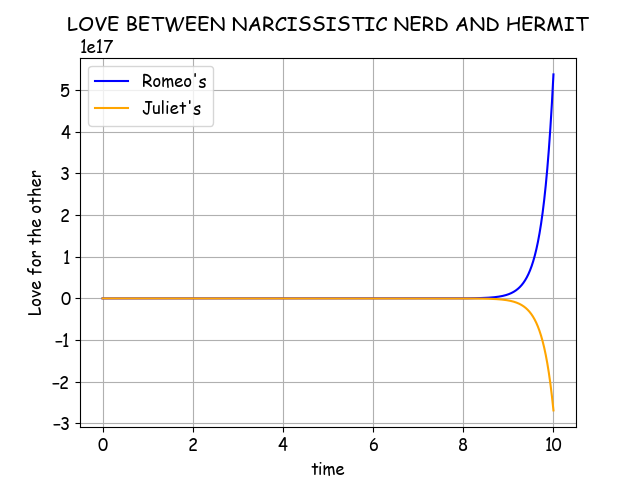
\includegraphics[width=100mm]{image/bt2/plot9.1.png}
    \caption{VD9.1 - The plot of the love between Narcissistic Nerd and Cautious Lover}
\end{figure}
\begin{figure}[!htbp]
    \centering
    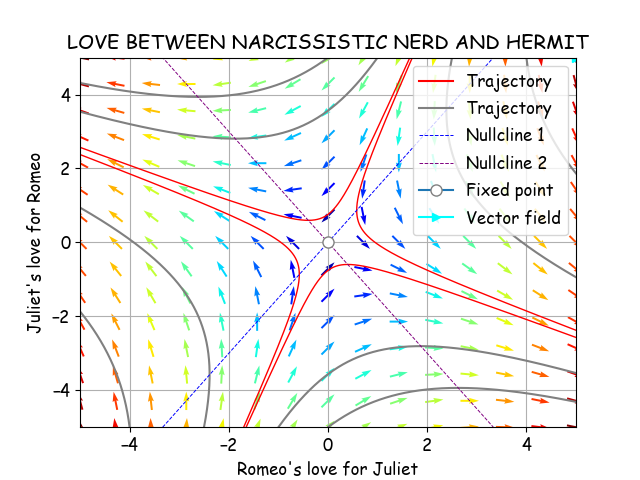
\includegraphics[width=100mm]{image/bt2/pp9.1.png}
    \caption{VD9.1 - The phase portrait of the love between Narcissistic Nerd and Hermit}
\end{figure}

\textbf{Dạng Phase portrait: } Saddle
\pagebreak
\begin{figure}[!htbp]
    \centering
    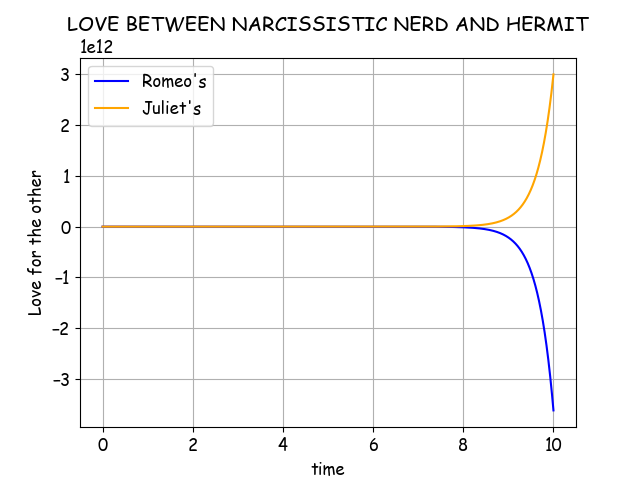
\includegraphics[width=100mm]{image/bt2/plot9.2.png}
    \caption{VD9.2 - The plot of the love between Narcissistic Nerd and Hermit}
\end{figure}
\begin{figure}[!htbp]
    \centering
    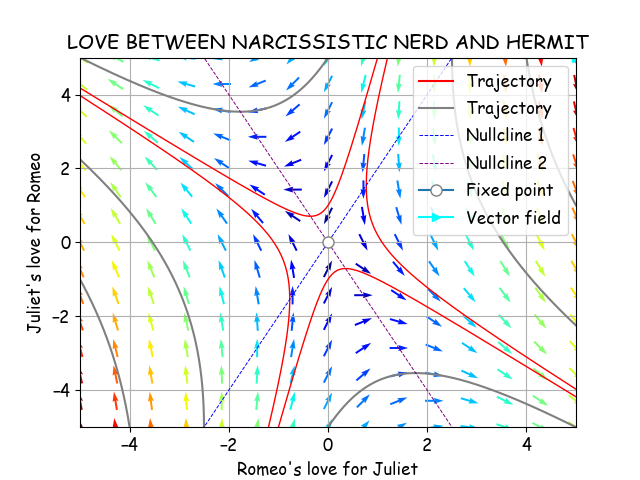
\includegraphics[width=100mm]{image/bt2/pp9.2.png}
    \caption{VD9.2 - The phase portrait of the love between Narcissistic Nerd and Cautious Lover}
\end{figure}

\textbf{Dạng Phase portrait: } Saddle
\pagebreak
%%%%%%%%%%%%%%%%%%101010101010%%%%%%%%%%%%%%%%%%%%%%%%
%%%%%%%%%%%%%%%%%%%%%%%%%%%%%%%%%%%%%%%%%%%%%%%%%%%%%
\begin{tcbdoublebox}[title={10. Cautious Lover and Hermit}]
\mdseries .\\
\bfseries Ví dụ 1: \\
\textcolor{blue}{$$\left\{\begin{matrix}
\dot{R} =  -2R +3J \\ 
\dot{J} =  -R-2J\\ 
R(0)= -\frac{12}{5}, J(0)=-\frac{9}{5}
\end{matrix}\right.$$}\\
\mdseries Ma trận $\color{blue}A=\begin{pmatrix}
-2 & 3\\ 
-1 & -2
\end{pmatrix}$ có hai trị riêng là 
$\color{blue}\lambda_{1}=-2+\sqrt{3}i;\ \lambda_{2}=-2-\sqrt{3}i$
, lần lượt tương ứng với các vecto riêng:
$\color{blue}v_{1} = (-\sqrt{3}i;\ 1)^{T};\ v_{2}=(\sqrt{3}i;\ 1)^{T}$\\Áp dụng công thức bài tập 1, nghiệm của hệ phương trình là:
$$R(t)=-\frac{12\,{\mathrm{e}}^{-2\,t}\,\cos\left(\sqrt{3}\,t\right)}{5}-\frac{9\,\sqrt{3}\,{\mathrm{e}}^{-2\,t}\,\sin\left(\sqrt{3}\,t\right)}{5}$$
$$J(t)=\frac{4\,\sqrt{3}\,{\mathrm{e}}^{-2\,t}\,\sin\left(\sqrt{3}\,t\right)}{5}-\frac{9\,{\mathrm{e}}^{-2\,t}\,\cos\left(\sqrt{3}\,t\right)}{5}$$
\\
\bfseries Ví dụ 2:\\
\textcolor{blue}{$$\left\{\begin{matrix}
\dot{R} = -6R -J \\ 
\dot{J} =  4R -2J\\ 
R(0)= -7, J(0)=4
\end{matrix}\right.$$}
\mdseries Ma trận $\color{blue}A=\begin{pmatrix}
-6 & -1\\ 
4 & -2
\end{pmatrix}$ có trị riêng bội hai là 
$\color{blue}\lambda_{1}=\lambda_{2}=-4$
, tương ứng với vecto riêng:
$\color{blue}v = (-1;\ 2)^{T}$\\Áp dụng công thức bài tập 1, nghiệm của hệ phương trình là:
$$R(0)=10\,t\,{\mathrm{e}}^{-4\,t}-7\,{\mathrm{e}}^{-4\,t}$$
$$J(t)=4\,{\mathrm{e}}^{-4\,t}-20\,t\,{\mathrm{e}}^{-4\,t}$$

\end{tcbdoublebox}
\pagebreak
\begin{figure}[!htbp]
    \centering
    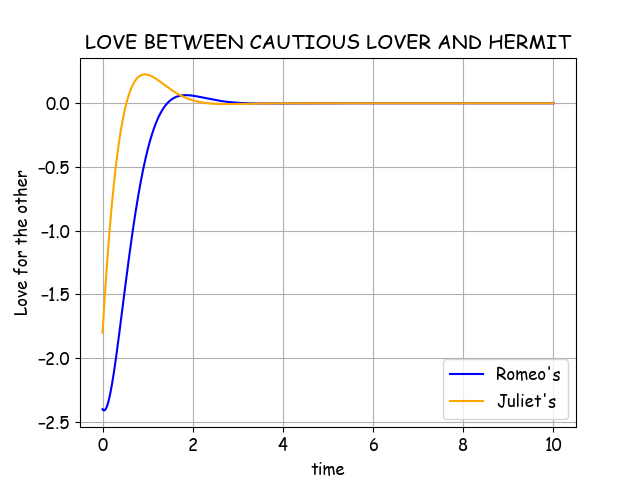
\includegraphics[width=100mm]{image/bt2/plot10.1.png}
    \caption{V10.1 - The plot of the love between Cautious Lover and Hermit}
\end{figure}
\begin{figure}[!htbp]
    \centering
    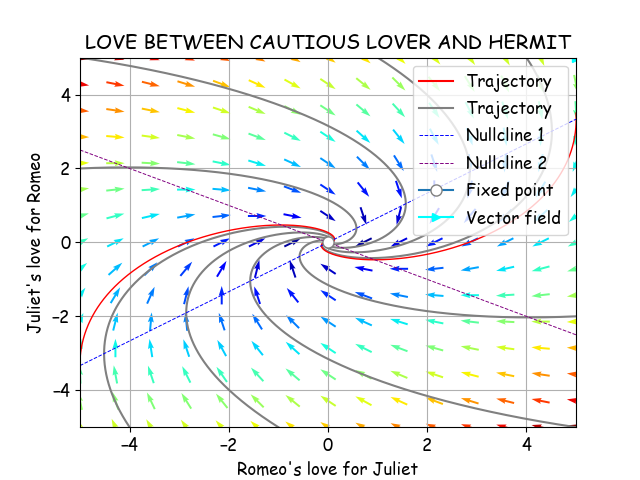
\includegraphics[width=100mm]{image/bt2/pp10.1.png}
    \caption{VD10.1 - The phase portrait of the love between Cautious Lover and Hermit}
\end{figure}

\textbf{Dạng Phase portrait: } Spiral Sink
\pagebreak
\begin{figure}[!htbp]
    \centering
    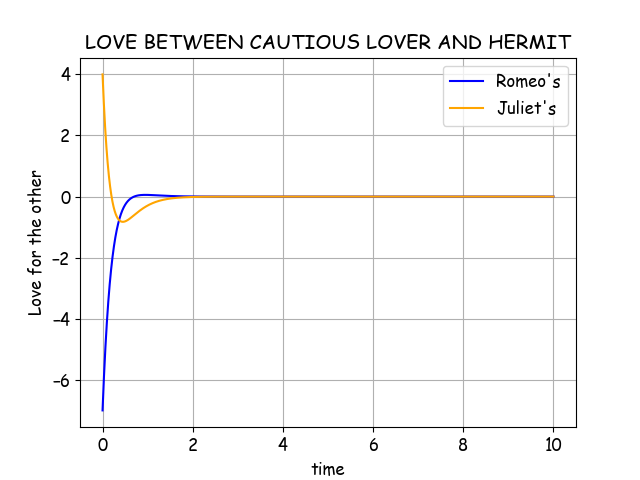
\includegraphics[width=100mm]{image/bt2/plot10.2.png}
    \caption{VD10.2 - The plot of the love between Cautious Lover and Hermit}
\end{figure}
\begin{figure}[!htbp]
    \centering
    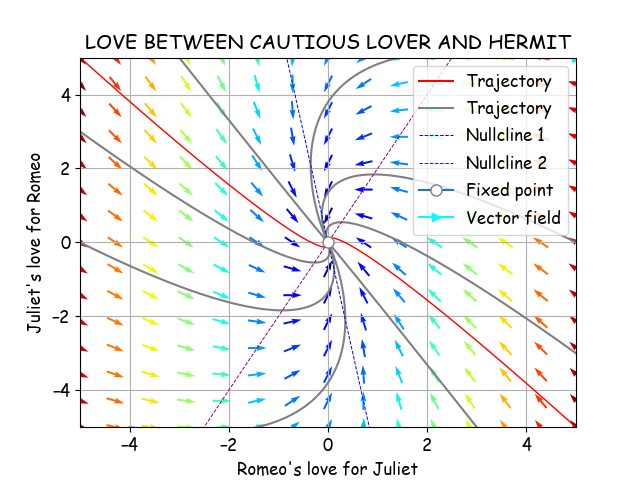
\includegraphics[width=100mm]{image/bt2/pp10.2.png}
    \caption{VD10.2 - The phase portrait of the love between Cautious Lover and Hermit}
\end{figure}

\textbf{Dạng Phase portrait: } Degenerate Nodal Sink
\pagebreak